\begin{exo}
	Dans le repère orthonormé $\OIJ$ ci-dessous, on considère le carré $ABCD$ et le parallélogramme $EFDC$.
	\begin{center}
		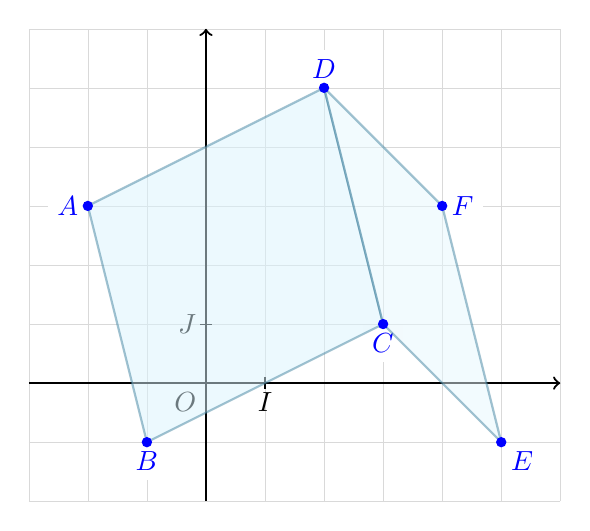
\begin{tikzpicture}[scale=0.75]
			\draw[gray!30, very thin] (-3,-2) grid (6,6);
			\draw[->, thick] (-3,0) -- (6,0);
			\draw[->, thick] (0,-2) -- (0,6);
			\node at (0,0) [below left] {$O$};
			\node at (1,0) [below] {$I$};
			\node at (0,1) [left] {$J$};
			\draw (1,-0.1) -- (1,0.1);
			\draw (-0.1,1) -- (0.1,1);
			\coordinate (A) at (-2,3);
			\coordinate (B) at (-1,-1);
			\coordinate (C) at (3,1);
			\coordinate (D) at (2,5);
			\coordinate (E) at (5,-1);
			\coordinate (F) at (4,3);
			\foreach \p/\name/\pos in {A/A/left, B/B/below, C/C/below, D/D/above, E/E/below right, F/F/right} {
					\node[\pos, blue, fill=white] at (\p) {$\name$};
				}
			\draw[thick, cyan!60!black, fill=cyan!15, opacity=0.5] (A) -- (B) -- (C) -- (D) -- cycle;
			\draw[thick, cyan!60!black, fill=cyan!10, opacity=0.5] (E) -- (F) -- (D) -- (C) -- cycle;
			\foreach \p/\name/\pos in {A/A/left, B/B/below, C/C/below, D/D/above, E/E/below right, F/F/right} {
					\fill[blue] (\p) circle (2.5pt);
				}
		\end{tikzpicture}
	\end{center}

	\begin{enumerate}
		\item Lire les coordonnées de tous les points.
		\item Calculer les coordonnées du milieu $K$ de $[AE]$.
		\item Calculer les coordonnées du milieu $L$ de $[BF]$.
		\item En déduire la nature du quadrilatère $AFEB$.
		\item Que dire alors des droites $(AF)$ et $(BE)$ ?
	\end{enumerate}
\end{exo}

